\chapter{Technischer Hintergrund}

\section{Vorgeschlagene Lösung}

\subsection{Kommunikation im Projekt Radig}
Im Projekt Radig ist keine echte Kommunikation zwischen dem Client und dem Server
vorhanden.

Die auf der Webseite dargestellten Werte werden vor dem senden der HTML-Seite
im HTML-Code eingefügt indem Platzhalter im Format "`\%PORTA0"' ersetzt und so statisch auf
der Webseite dargestellt werden. Das Manipulieren der Pins findet über ein HTML-Formular
statt. Alle manipulierbaren Pins sind als Input vom Typ Checkbox dargestellt. Diese lassen
sich frei manipulieren und erst beim Betätigen des "`Senden"'-Buttons werden die
Informationen per POST-Event an den Server gesendet und so die Seite neu aufgerufen. Der
Server filtert die POST Informationen aus dem HTTP-Header und manipuliert die Pins gemäß
den Anweisungen. Beim senden des angeforderten HTML-Dokumentes werden die neuen Werte in
den HTML-Code eingefügt, und so die neuen Werte auf der Webseite angezeigt.

Das große Problem bei dieser technisch einfachen Lösung ist, das geänderte Werte erst beim
nächsten neu laden der Webseite angezeigt werden. Ändert sich ein Pin während die Webseite
dargestellt wird bekommt der Nutzer dies nicht mit. Zudem wird bei jedem Manipulieren
eines Pins die gesamte Seite neu geladen und so Unmengen an unnötigen Daten übertragen.
Auch zum darstellen der aktuellen Werte muss die ganze Seite neu vom Server angefordert
werden.

\subsection{Erster Ansatz}
Die Kommunikation zwischen Server und Client sollte mit Hilfe einer REST-Schnittstelle
stattfinden, die im Hintergrund über Javascript angesprochen werden kann.

Eine REST-Schnittstelle besteht aus einer oder mehreren virtuellen URLs. Beim Aufruf einer
solchen URL liefert der Server kein Dokument das gespeichert ist, sondern erzeugt
dynamisch eine Antwort mit den benötigten Informationen und sendet diese als Antwort
zurück. Der Server kann beim Aufruf einer URL auch eine Aktion ausführen.

Vorteile der REST-Schnittstelle ist die simple Implementierung, sowohl auf dem Client mit
JavaScript als auch auf dem Server. Die Inhalte werden mit JSON formatiert, welches einen
technisches Standart darstellt und sich in JavaScript direkt in ein Objekt umwandeln
lässt. Auf dem Server ist es einfach mit einem Stringformat immer gleiche JSON Strukturen
zu erstellen und nur aktuelle Werte einzufügen. Die REST-Schnittstelle lässt sich leicht
um weitere, neue Funktionalitäten erweitern, indem neue virtuelle URLs erstellt werden die
vom Client ansprechbar sind.

Die Anforderungen an eine Lösung in diesem Projekt waren vor allem eine möglichst kompakte
Schnittstelle zu schaffen die wenig Bandbreite verbraucht um eine hohe
Übertragungsgeschwindigkeit zu ermöglichen trotz des schwachen Servers. Ein besonderes
Augenmerk war auf die Übertragung der Messwerte zu legen, da diese nicht wie andere
statische Informationen nur einmalig übertragen werden sondern kontinuierlich erneuert
werden müssen. Die Schnittstelle sollte gut skalierbar sein. Würde später ein Port für
eine andere Aufgabe zu verwendet werden muss dieser Port ohne Aufwand aus der
REST-Schnittstelle ausgeschlossen werden können, damit er von außen nicht manipulierbar
ist und so interne Abläufe auf der Platine nicht gestört werden.

Nach den Anforderungen muss die Schnittstelle folgende Aufgaben ermöglichen:
\begin{itemize}
  \item Abfragen der aktuellen Werte aller verwendbaren Pins
  \item Abfragen der Konfiguration eines Pins (Eingang oder Ausgang)
  \item Abfragen von Allgemeinen Informationen des Boards (IP, Standart-IP, Mac-Adresse,
  Serverversion)
  \item Manipulieren aller als Ausgänge geschaltener Pins
  \item Manipulieren der Konfiguration eines Pins (als Eingang oder Ausgang setzen)
  \item Manipulieren von Servereinstellungen (z.B. IP-Adresse);
\end{itemize}

%\begin{itemize}
%	\item Aufbau als REST-Schnittstelle
%	\begin{itemize}
%		\item Simpel implementierbar
%		\item Technischer Standart
%		\item Fertige Mechaniken in JavaScript
%		\item Leicht erweiterbar um neue Funktionalitäten
%	\end{itemize}
%	\item Anforderungen an eine Lösung:
%	\begin{itemize}
%		\item Möglichst kompakt, wenig Bandbreite soll verbraucht werden
%		\item Messwerte müssen besonders effizient übertragen werden
%		\item Skalierbar - Egal ob ein oder 20 Ports verwendet werden
%		\item Neben Abfragen der Messwerte auch manipulieren der IP, des DDR und der
%			  Ausgänge
%		\item JSON-Encodiert, direkt in JavaScript Objekt überführbar
%	\end{itemize}
%\end{itemize}

%-----------------------------------------------------------------------------------------
\subsection{Polling oder Pushing}
Die aktuellen Werte der Pins müssen bei jeder Änderung vom Server zum Client übertragen
werden, damit diese auf der Webseite immer korrekt dargestellt werden. Hierfür stehen zwei
verschiedene Konzepte zur Verfügung wie die Übertragung der Daten initialisiert werden.

\subsubsection{Polling}
Bei Polling werden vom Client kontinuierlich die Werte erneut angefordert, indem dieser
die entsprechende virtuell URL des Servers aufruft. Dies führt dazu, dass viele unnötige
Date übertragen werden, da sich eventuell nicht bei jedem erneuten anfordern der Werte
diese auch tatsächlich verändert haben und so die gleichen Datensätze oft mehrmals
angefordert werden.

Im Vergleich zu der Radig-Lösung bietet Polling den Vorteil das die Werte kontinuierlich
nach geladen und so immer korrekt dargestellt werden während die Webseite dargestellt
wird. Auch das gesendete Datenvolumen wird dahingehend minimiert, das nur die Nutzdaten
übertragen werden und nicht der gesamte HTML-Code der Webseite. Polling ist technisch sehr
einfach zu realisieren, da die Abfrage der Daten einfach zyklisch wiederholt werden.

\subsubsection{Pushing}
Bei Pushing wird im Gegensatz zu Polling der Daten nicht vom Client initialisiert sondern
vom Server. Der Server weiß wann sich die Werte geändert haben und kann dem Client bei
jeder Änderung gezielt die neuen Daten übermitteln. Das Übertragen der Daten
könnte z.B. durch einen Interrupt ausgelöst werden.

Im direkten vergleich zu Polling bietet Pushing verschiedene Vorteile. So wird nicht nur
das Volumen der übertragenen Daten reduziert indem keine unnötigen Abfragen stattfinden,
sondern die neuen Werte gelangen auch genau dann zum Client wenn die Änderung tatsächlich
stattgefunden hat, was dazu führt das die Webseite schneller auf Änderungen reagiert.

Die technische Umsetzung von Pushing ist mit diversen Problemen verbunden. Die typische
Verbindungsaufbaurichtung ist bei Webanwendungen und Webseiten immer vom Client zum
Server. Anders als bei Polling müssen bei Pushing Daten vom Server zum Client gelangen.
Hierfür muss eine Verbindung vom Server zum Client aufgebaut werden. Dies ist technisch
aber nicht möglich, da der Browser bzw. JavaScript keine Möglichkeit haben einen Port des
Clientsystems zu öffnen und auf eingehende Verbindungen des Servers zu antworten.

Das Problem lässt sich durch die Benutzung von HTML5 Server-Sent Events umgehen. Hierbei
frägt der Client eine virtuelle URL des Servers ab, ähnlich einer REST-Schnittstelle. Der
Server überträgt jedoch nicht sofort Daten, sondern schreibt erst bei einem Event (z.B.
die Änderung eines Pins) in den geöffneten Stream und pusht so die Daten zum Client.
Dieser überwacht den Stream mit Hilfe von JavaScript un empfängt so die neuen Werte und
kann sie auf der Webseite anzeigen.

Dieses System ist auf dem Pollin Net-IO Board aber nur schwer umzusetzen da mehrere
Verbindungen verwaltet werden müssen. So ist immer mindestens eine Server-Sent Event
Verbindung offen, parallel könnte aber ein Client andere Daten vom Server anfordern. Für
das Verwalten mehrerer Verbindungen sind aber viele Resourcen nötig, da für jede
Verbindung auch Daten im RAM hinterlegt werden müssen. Außerdem st in vielen Situationen
ein simples Multitasking nötig, das so auf einem ATmega CPU nicht vorhanden ist. Das Radig
Projekt setzt aus diesen Gründen auf HTTP 1.0 bei dem für jede Anfrage eine Verbindung
geöffnet und nach erfolgreichem Übertragen der Daten wieder geschlossen wird. So ist auch
die Kommunikation mit mehreren Clients problemlos möglich.

\subsubsection{Entscheidung}
Pushing ist leider nur schwer umsetzbar auf dem Microcontroller. Dies ist
bedingt durch die knappen Resourcen wie Arbeitsspeicher, als auch durch das nur
schwer umsetzbare Multitasking, das für einen reibungslosen Ablauf nötig ist. Ohne Multitasking
ist nicht gewährliestet das alle Dateien übertragen werden können, da der
Server, sobald eine Server-Sent Event Verbindung aufgebaut wird, nicht mehr
verfügbar ist, bis diese wieder geschlossen wird. Eine Benutzung durch mehrere
Clients ist so nicht denkbar und auch die Nutzung von nur einem Client kann zu
Problemen führen wenn dieser Daten anfordert nachdem die Server-Sent Event
Verbindung aufgebaut worden ist.

Die Implementierung von Multitaskign ist zwar prinzipiell möglich, erfordert
aber einen tiefen Eingriff in das Vorlagenprojekt, da neben der eigentlichen
Nebenläufigkeit zusätzlich der gesamte Server threadsafe gestaltet werden
müsste.

Aus diesen Gründen entschlossen wir uns das technisch unsauberere Polling zu
verwenden, da die Implementierung von Pushing den Rahmen des Projektes
übersteigen würde.

%-----------------------------------------------------------------------------------------
\subsection{Aufbau der Server-Kommunikation}

Bei der Server-Kommunikation gibt es zwei grundsätzliche Kanäle:
\begin{itemize}
  \item Das Abfragen von Daten beim Server
  \item Das Manipulieren von Servereinstellungen (z.B. Pinwerte)
\end{itemize}
Das Manipulieren von Servereinstellungen war bereits im Projekt Radig möglich.
Hierfür interpretiert der Server die POST-Parameter jeder Anfrage und setzt ggf.
die Pins neu. Für die neuen Anforderungen wie das Manipulieren des DDR haben
wir und dazu entschlossen den bereits vorhandenen Code nur leicht zu
manipulieren und zu erweitern.

Für das Abfragen von Daten ist im Projekt Radig keine Lösung vorhanden, da hier
die Werte statisch in Form von Platzhaltern im HTML-Text eingebunden sind und
beim Abfragen der HTML-Datei durch die Werte ersetzt werden. Folglich muss die
gesamte Seite erneut geladen werden, um die dargestellten Werte zu
aktualisieren. Um dies zu vermeiden haben wir uns entschlossen die Daten
dynamisch abzufragen, um sie gesondert von der Webseite laden zu können.

\subsubsection{Mögliche Techniken für Datenabfrage}

Für die dynamische Datenabfrage gibt es veschiedene Standards. Hierzu gehöhren
verscheidene \ac{XML}-Basierte Protokolle wie RSS, als auch das so genannte
\ac{REST}.

\ac{XML}-Basierte Protokolle wie \ac{RSS} oder \ac{SOAP} weisen typischerweise
einen großen Protokoll-Overhead auf und sind deswegen nur bedingt für den Einsatz auf einem
Microcontroller geeignet, da das System zu viel unnötige Daten übertragen
müsste. Außerdem muss das dynamische \ac{HTTP}-Abfragen der Daten per JavaScript
erfolgen, welches die in \ac{XML} präsentierten Daten erst wieder parsen müsste, was
zusätzlichen Code auf dem Client bedeuten würden.

\ac{REST} hingegen präsentieren die Daten in \ac{JSON}, welches von
JavaScript direkt als Objekt interpretiert werden kann. Dies erspart das
aufwendige parsen der Daten. Außerdem ist der Protokoll-Overhead bei \ac{JSON}
tendenziell kleiner als bei \ac{XML}-Basierten Lösungen, da weniger lange Tagnamen
vorhanden sind, was eine effektievere Übertragung ermöglicht.

Aus diesen Gründen haben wir uns für eine \ac{REST} Lösung entschieden.

\subsubsection{Design der REST-Schnittstelle}
Bei \ac{REST} gibt es für jede Abfrage eine seperate \ac{URL}. Bei uns liegen
alle URLs im Unterverzeichnis \textrm{/rest}. Insgesamt gibt es 3 URLs:
\begin{itemize}
  \item  \textrm{/rest/info} liefert generelle, statische Informationen über den
  Server, wie z.B. die Server-Version
  \item  \textrm{/rest/pininfo} liefert generelle, statische Informationen über
  die einzelnen Pins, wie z.B. den Namen des Pins
  \item  \textrm{/rest/valus} liefert nur die aktuellen Werte und
  \ac{DDR}-Einträge.
\end{itemize}

Um die dargestellten Werte auf der Webseite zu aktualisieren muss folglich nur
\textrm{/rest/valus} erneut geladen werden. Aus diesem Grund sollte diese
Datei so klein wie möglich gehalten werden um eine optimale
Aktualisierungsgeschwindigkeit zu ermöglichen. \textrm{/rest/info} und  
\textrm{/rest/pininfo} müssen nur einmalig geladen werden, da die enthaltenen
Informationen statisch sind und nie geändert werden. Die Größe dieser Dateien
ist deshalb weniger ausschlaggebend.
%-----------------------------------------------------------------------------------------
\subsection{Implementierung der REST-Schnitstelle auf dem Server}
Für die Implementierung der \ac{REST}-Schnittstelle setzen wir auf dem
besethenden Code aus dem Projekt Radig auf. Typischerweise sind
\ac{REST}-\ac{URL}s virtuelle \ac{URL}s.
Das bedeuted das unter dieser \ac{URL} keine Datei vorhanden ist, sondern diese bei
bedarf dynamisch erzeugt werden. Um die Implementierung möglichst einfach zu
halten haben wir uns dazu entschlossen unter der gegebenen \ac{URL} (also z.B  
\textrm{/rest/values}) eine mit Platzhaltern versehene Datei abzulegen. Das
Vorgehen mit Platzhaltern wurde schon im Projekt Radig verwendet um die
Informationen in den statischen \ac{HTML}-Code einzufügen. Die Platzhalter
werden vor dem Senden der Datei durch zugehörige Werte ersetzt.\\
\\
Das Schema für so einen Platzhalter ist \textrm{\%PINXY} und setzt sich zusammen aus dem
Aufruf \textrm{\%PIN}, dem anzusprechendem Port X = [A,C oder D] und dem Pin Y = [0-7] (z.B.
\textrm{\%PINC1 } ). Mit diesem Platzhalter kann der direkte Pin Ausgelesen
(Hier Port C und Pin 1) und an eine beliebige Stelle im Quellcode platziert werden. Neu
hinzugekommen ist das Ausgeben der Information ob der Konkrete Pin über das
DDRegister als Ein- oder Ausgang definiert ist. Das Schema ist für diesen
Platzhalter ist \textrm{\%DDRXY} und setzt sich zusammen aus dem Aufruf \textrm{\%DDR}, dem
anzusprechendem Port X = [A,C oder D] und dem Pin Y = [0-7] (z.B.
\textrm{\%DDRD1} ). 

%-----------------------------------------------------------------------------------------
\subsection{Erweiterung der POST-Parameter}
Um Manipulationen an dem Board vorzunehemen haben wir uns entschlossen das
vorhandenen System zu erweitern. Hierbei werden bei jeder \ac{HTTP}-Anfrage die
POST-Parameter ausgewertet und das Board entsprechend manipuliert.\\
\\
Das setzen der Ausgänge wird über einen HTTP-Post Aufruf getätigt. So können die
Pins des entsprechenden Ports gesetzt oder umgeschaltet werden. Die
Informationen, die zum setzen eines Ports benötigt werden setzen sich zusammen
aus einem \textrm{SET} Befehl und dem Aufruf PORTXYZ zum setzen oder dem
\textrm{SET} Befehl und dem Aufruf OUTXYZ. X steht für den anzusprechendem Port
X = [A,C oder D]. Y und Z Stehen für die Einstellung der Pins in hexadezimaler
Schreibweise (00-FF) Abschließend muss das Ende der Schaltanweisung mit
\textrm{SUB} gekennzeichnet werden, da der Webserver auf diese Steuerzeichen
prüft. Ein Beispiel Post zum setzen der Pins C0-C3 auf Ein, der Pins C4-C7 auf
Aus, dem umschalten der Pins D0-D3 als Ausgang und der Pins D4-D7 als Eingang
sieht folgendermaßen aus:
\\

\framebox{SET=PORTC0F\&SET=OUTD0F\&SUB=Senden}

%-----------------------------------------------------------------------------------------

\subsection{Implementierung der REST-Schnitstelle auf dem Client}
Auf der Webseite müssen die vom Server bereitgestellten \ac{REST}-URLs im
Hintergrund aufgerufen werden können. Hierzu verwendeden wir die bereits in JavaScript
enthaltene \ac{AJAX} Bibliothek. \ac{AJAX} erlaubt JavaScript URLs im
Hintergrund zu laden, ohne das der Nutzer dies bemerkt oder die Seite neu geladen wird. 

\begin{figure}[H]
\lstinputlisting[language=JavaScript]{content/code/ajaxexample.js}
\caption{JavaScript um \textrm{/rest/valus} abzufragen und in ein Objekt zu
parsen}
\label{Ein typischer AJAX-Request}
\end{figure}

Der hier beispielhaft gezeigte Quelltext ermöglicht das laden der \ac{URL}
\textrm{/rest/valus}.
Hierfür wird ein XMLHttpRequest-Objekt verwendet und der geladene Text
(\textrm{x.responseText}) wird mit \textrm{JSON.parse(\ldots)} in ein
JavaScript-Objekt verwandelt.

Sämtliche Server-Kommunikation findet ausschlißlich in \textrm{rest.js} statt.
Hier werden Methoden zum ansprechen des Servers bereit gestellt, welche überall
verwendet werden können ohne Netzwerkcode zu schreiben. Um beliebige Dateien
abzufragen gibt es die Methoden \textrm{loadURL(url)} und
\textrm{loadURLAsync(url, postParams, func)}. \textrm{loadURL(url)} lädt die
Datei synchron und gibt den erhaltenen Text zurück. Das synchrone Laden
bedeutet, das der Aufruf dieser Methode das Programm blockiert, bis die Datei
vollständig geladen wurde. \textrm{loadURLAsync(url, postParams, func)} hingegen
lädt die Datei asynchron im Hintergrund. Sobald das Laden abgeschlossen ist wird
die als Parameter übergebene Funktion \textrm{func} aufgerufen.
\textrm{loadURLAsync(url, postParams, func)} kann außerdem ein Text als
POST-Parameter übergeben werden. Dies ermöglicht das Manipulieren des Boards
über die POST-Parameter, welche vom Board interpretiert werden.

\textrm{rest.js} ruft \textrm{loadURLAsync(\ldots)} in einer festen Frequenz
kontinuirlich auf. Nach jeder aktualisierung wird eine Funktion aufgerufen,
welche über die Methode \textrm{setOnValuesChanged(func)} gesetzt werden kann.

Alle von \textrm{rest.js} zur Verfügugn gestellten Funktionen sowie deren
Verwendung sind der ausführlichen Sourcecode-Dokumentation zu entnehmen.
%\begin{itemize}
%  \item Aufruf der URLs im Hintergrund mit Ajax
%  \item info und pininfo werden zu Beginn einmalig aufgerufen (synchron um zu
%  gewährleisten das die Daten zur Verfügung stehen für andere Initialisierungen)
%  \item values wird mit setTimeout(...) zyklisch assynchron aufgerufen
%  \item synchrones aufrufen von values führt dazu, das sich die Webseite aufhängt, da
%  der (Single-)JavaScript Thread mit dem laden der Daten beschäftigt ist und nicht
%  für andere Aufgaben zur Verfügung steht. Bei einem assynchronen Aufruf werden
%  die Daten von einem anderen Thread im Hintergrund geladen
%  \item JSON-Text wird mit JSON.parse(...) in ein Objekt transformiert
%  \item Informationen werden über entsprechende getter zur Verfügung gestellt
%  \item Funktion onValueChanged wird jedes mal aufgerufen wenn neue Daten zur
%  Verfügung stehen
%  \item onError wird aufgerufen wenn ein Fehler in der Kommunikation aufgetreten ist
%  \item Über setter werden die entsprechenden URLs assynchron aufgerufen und so
% die  Daten an den Server übermittelt
%\end{itemize}

%-----------------------------------------------------------------------------------------

\section{Werkzeuge}

%-----------------------------------------------------------------------------------------
\subsection{Das Atmel Studio}

Das Atmel Studio ist als \ac{IDE} das zentrale Werkzeug um einen Mikrocontroller
zu programmieren Dabei ist das Atmel Studio, welches von Atmel nach einer
Kostenlosen Registrierung beziehbar ist, stark an die Microsoft Visual \ac{IDE}
angelehnt. Wenn man bereits Erfahrungen mit Visual Studio gesammelt hat, wird
man sich schnell im Atmel Studio zurecht finden. Zu den Reinen
Programmierwerkzeugen gibt es im Atmel Studio noch ein paar weiter Funktionen
die das Arbeiten mit den Mikrocontroller erleichtert.


\subsubsection{Device Programming}
\label{Chap:atmelStudio.Programming}

Eine Kernkomponente beim Atmel Studio ist das Device Programming Fenster.
Erreicht werden kann es über "`Tools $\to$  Device Programming"'.
Hier kann die Aktuelle Verbindung mit dem Microcotroller getestet werden. Die
Einstellungen werden hier aus den Projekt Einstellungen entnommen können aber
auch frei gewählt werden. Dazu gehören: das Momentan
angeschlossenen Programmier Werkzeugs, dem Verwendeten Mikrocontroller und der
Schnittstelle. Durch drücken der Read Buttons kann die Korrektheit der
Verbindung geprüft werden. Wenn es zu keiner Fehlermeldung kommt und die Ziel
Spannung bei ungefähr 5V liegt ist der Mikrocontroller korrekt
angeschlossen.

\begin{figure}[H]
\centering
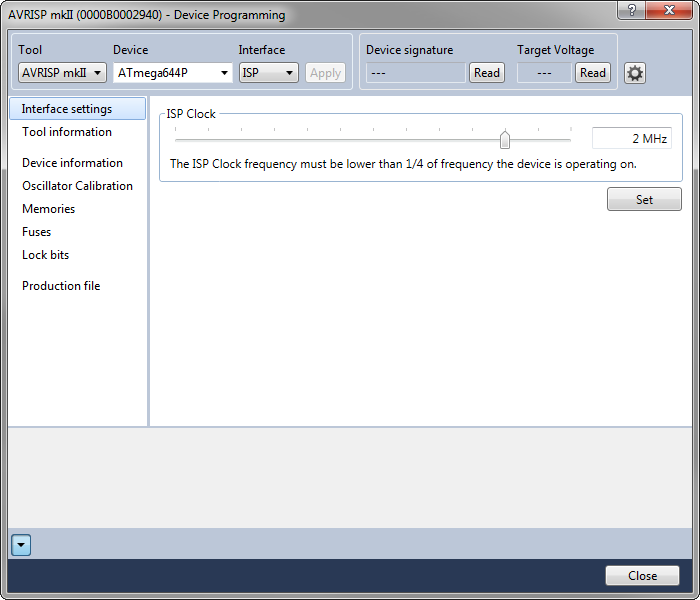
\includegraphics[width=13cm]{content/pictures/Anleitung/neuerProzessor/AnleitungNeuerProzessor1.png}
\caption{DeviceProgramming}
\label{fig:B3}
\end{figure}

Weiter können über den Abschnitt Fusebits die entsprechenden Fuse Einstellungen
getroffen werden, dazu mehr im Kapitel Fusebits \ref{chap:Fuse}


\subsubsection{Projekt Einstellungen}

Zur als weitere wichtige Einstellung für das Projekt sind die Projekt
Einstellungen. Hier kann das Werkzeug zum Programmieren, die Schnittstelle und
die Übertagungstakt gewählt werden.
Der Übertagungstakt sollte auf ungefähr 1 MHz gesetzt, damit er zum
einen nicht zu langsam und auch nicht zu schnell ist. Er darf nicht 1/8 des
Prozessortaktes überschreiten.

%Todo Projekteinstellungen grafik

%-----------------------------------------------------------------------------------------
\subsection{AVRDUDE}

Avrdude ist ein Alternatives Werkzeug zum Bearbeiten von Mikrocontrollern. Es
ist im Gegensatz zum Atmel Studio lediglich ein Konsolen Werkzeug ohne
grafische Oberfläche. Mit Avrdude können unter anderem die Fusebits von einem
Mikrocontroller gelesen und gesetzt werden. Weiter ist es möglich eine Sicherung
von dem Aktuellen stand des Mikrocontrollers herzustellen oder ein Hex Datei auf
den Mikrocontroller aufzuspielen. Avrdude unterstützt eine Reihe von \ac{ISP}
Geräten unter anderem auch den von uns verwendeten Atmel AVRISPmkII. Der Einsatz von
Avrdude war notwendig, da die Fusebits von einem Neuen Microcontroller
Standartmäßig auf den internen Quarz-Kristall gesetzt sind und nicht auf den
Externen Kristall des AVR-NET-IO Boards.
Eine genaue Anleitung gibt es im Kapitel \ref{chap:Benutzerhandbuch}
Benutzerhandbuch.

%-----------------------------------------------------------------------------------------
\subsection{HTML Header Compiler}
\label{chap:hintergrund.HHC}

Zum automatischen umwandeln der Quell-Dateien (html, js, png etc\ldots) haben
wir einen speziellen HTML Header Compiler entwickelt der die Website in eine
für den Webserver verständliche Headerdatei umwandelt. Der Compiler durchsucht
den Eingabe Ordner und sammelt die darin enthaltenen Dateien. Daraus entsteht
dann die für das Projekt benötigte Header Datei, bestehend einem Array von
Buchstaben für jede Datei. Der \ac{HHC} ist den Projektdateien, mit denen diese
Dokumentation ausgeliefert wurde beigelegt, kann aber auch zusammen mit dem
Projekt auf Github \url{https://github.com/doofmars/Embedded-Webserver}
bezogen werden.\\

Eine Beispiel Umwandlung: 

\begin{figure}[H]
\lstinputlisting[language=HTML]{content/code/index.html}
\caption{index.htm}
\label{HHC.input}
\end{figure}

Das eingegebene Verzeichnis, welches die \textrm{index.html} Datei enthält wird
eingelesen und in die folgende Headerdatei umgewandelt.
Abbildung \ref{HHC.input} zeigt eine simple "`Hallo Welt"' Website, die keine
weitere Funktion besitzt. Nachdem die Website mit dem HTML-Header-Compiler
umgewandelt wurde, entsteht die Headerdatei aus Abbildung \ref{HHC.output}. Gut
zu erkenne ist das Array aus Buchstaben in hexadezimaler Schreibweise welches die
index.html Datei widerspiegelt.
Am Ende der Headerdatei ist ein weiteres Array, bestehend aus Schlüssel-Wert
paaren für den Webserver. Hier wird hinterlegt welche Dateien vorhanden sind.
Der letzte Eintrag in diesem Array signalisiert das Ende der Suche und ist die
Bedingung für den Webserver um zur Standardausgabe zu wechseln. Bsp: Eine HTML
Datei wird angefordert die nicht existent ist, resultiert in der Ausgabe von
index.html.

\begin{figure}[H]
\lstinputlisting[language=C]{content/code/webpage.h}
\caption{webpage.h}
\label{HHC.output}
\end{figure}

Anzumerken ist das Standardmäßig der HTML Header Compiler die eingegebenen HTML
und JS Dateien optimiert in die Headerdatei speichert. Dazu wird die
Formatierung für den Zeilenvorschub, Tabulator oder Wagenrücklauf entfernt.
Falls dies für die Entwicklung nicht gewünscht ist, kann man diese Funktion
durch den Parameter \textrm{-n oder -newline} deaktivieren.
Außerdem ist die entstandene Headerdatei nicht zur Bearbeitung gedacht. Die
Bearbeitung erfolgt ausschließlich im Quelltext (z.B. der index.html). Analog
kann man dazu einen beliebigen Compiler einer herkömmlichen Programmiersprache sehen. Dieser
erzeugt aus dem Quelltext eine Binärdatei, diese ist nicht unbedingt
für Menschen lesbar. Bei Änderungen wird der Quelltext angepasst und neu
Compiliert. Da die Headerdatei folglich nicht bearbeitet werden muss haben wir
uns für eine Ausgabe als Array aus Buchstaben in hexadezimaler Schreibweise
entschieden, da es eine einfachere Programmatische Strukturierung erlaubt.

\subsection{AVRISPmkII}

Der AVRISPmkII ist ein einfacher \ac{ISP} Programmierer. Mit ihm ist es nur
möglich Programme auf den Mikrocontroller zu übertragen. Es ist nicht möglich
das Programm zu debuggen. Durch den Mangel der Debugfunktion ist der AVRISPmkII
relativ günstig und kann auch durch andere Baugleiche \ac{ISP} Programmer ersetzt
werden. Für den einfachen Anschluss mit dem AVR-Net-IO kann ein Adapter
angefertigt werden, zur Verbindung mit dem Computer nutzt der AVRISPmkII eine
USB Verbindung.

\subsection{AVRJTAGICEmkII}

Der AVRJTAGICEmkII ist ein ein Programmer der neben der \ac{ISP} Schnittstelle
zum Programmieren auch \ac{JTAG} unterstützt. Über das Atmel Studio ist es
einfach möglich mit \ac{JTAG} das Programm zu debuggen.
Der Anschluss von ISP oder JTAG wird im Benutzerhandbuch genauer erklärt.
